\chapter{Architectural Overview}
\label{ch:architectural_overview}
In this chapter, the architectural overview of the run-time state migration approach is discussed. We talk about the architecture that needs to be considered for implementation. Moreover, we stress about the chosen design pattern and its life cycles.

\section{Publish–subscribe pattern}
An infrastructure is needed to exchange run-time states of applications on different devices. Also, devices should know which other devices with common Application State Models are available and notice if they join or leave the network. Moreover, devices should be able to migrate the run-time state and acknowledge other devices when migration is done.

In this approach, we chose to use the publish-subscribe pattern. Thereby, the middleware is the message broker, devices are publishers, Application State Models are topics, and run-time states are messages. Also, there are extra topics and messages that allow us to fulfil requirements. 

\subsection{Topics}
There are some topics each device should subscribe to them. Devices whose subscribed to these topics receive a message if another device publish a message into them.

\subsubsection{Online}
All devices should subscribe to a topic about their connectivity status. This topic is \lstinline[basicstyle=\ttfamily]{online}. If a device joins or leaves the network, other devices get notice by a message.

\subsubsection{Application State Models}
Each Application State Model has a topic. Devices that supports these Application State Models should subscribe to these topics. So, If a device joins the same topic, it should notify other devices about joining and supporting the same Application State Model and also other devices notify the new device about their existence as a response. Also, for each Application State Model, devices should subscribe to the topic of Application State Models and a subtopic of device identification, that they can receive an individual message from other devices and vice versa. As users may use different devices and applications device identification must be unique like UUID; but in examples for readability reasons we use name of the device and application.

\subsubsection{Example Scenario}
Considering the scenario of Figure \ref{fig:asml-overview}. Three devices share some Application State Models. All devices should subscribe to \lstinline[basicstyle=\ttfamily]{online} topic. Mailspring supports three Application State Models, so it should subscribe to topics:
\begin{verbatim}
online
search
new-event
sending-email
\end{verbatim}

Also, to guarantee that other devices on the same topic can send message to Mailspring, it should subscribe to these subtopics with its identification: 
\begin{verbatim}
search/mac-mailspring
new-event/mac-mailspring
sending-email/mac-mailspring
\end{verbatim}

As K-9 Mail supports two Application State Models, it has to subscribe to these topics:
\begin{verbatim}
online
search
sending-email
search/android-k9mail
sending-email/android-k9mail
\end{verbatim}


Also, as Woven supporting one Application State Model, it has to subscribe to these topics:
\begin{verbatim}
online
new-event
new-event/windows-woven
\end{verbatim}

So, if K-9 Mail and Woven are already in the network and Mailspring joins, it  sends a message to topics \lstinline[basicstyle=\ttfamily]{search}, \lstinline[basicstyle=\ttfamily]{sending-email} and \lstinline[basicstyle=\ttfamily]{new-event} which allows K-9 Mail and Woven get notify about joining the new device with common Application State Models. Also, Woven sends back a introduction response message to \lstinline[basicstyle=\ttfamily]{new-event/mac-mailspring} about its existence. Morever, K-9 Mail should do the same but to \lstinline[basicstyle=\ttfamily]{search/mac-mailspring} and \lstinline[basicstyle=\ttfamily]{sending-email/mac-mailspring} topics.


\subsection{Events}
In this architecture, we need some events to fulfill our requirements.
\subsubsection{Device Introduction}
When a user runs an application, the application should introduce itself to other devices on the network. Moreover, other devices should get notify and response with their introduction.

As each application and platform has different life cycle and entry points, this event is part of the glue code and needs to be coupled with the application.

\subsubsection{Device Leave}
After an application got closed or a device went offline, it should notify other devices about this event. Moreover, other devices should not be able to communicate with that device.

\subsubsection{Device Has Run-time State}
If a device has a run-time state, it should notify other devices which support  common Application State Model.

\subsubsection{Store Run-time State}
If a device has a run-time state, it should be stored if other devices request the run-time state migration.

\subsubsection{Request Run-time State}
A device can request a run-time state of other devices supporting the common Application State Model. The target device should respond to this request.

\subsubsection{Send Run-time State}
As the source device can request a run-time state, the target device should respond to this request by sending its run-time state. Also, the source application should be aware of receiving it.

\subsubsection{Run-time State Migration}
After the target device received a run-time state and is adjusted into the application, the target device should notify the source device about finalizing the run-time state migration to react to this event.


\section{Middleware}
If devices are not on the same network, a middleware shall exist in which applications can communicate with each other. Figure \ref{fig:solution-overview} shows the role of middle-ware.
This middleware can handle sending and receiving the run-time state.
The goal of having this middleware is applications which coupled with
libraries, can introduce themselves, find each other, and migrate the run-time state.

Also, as mentioned in \textbf{R4 Device Management}, middleware is responsible for device discovery and notifying other devices if a device joins or leave with the same Application State Model.

As in this thesis, we considered the publish-subscribe pattern as the architecture, middleware is the intermediary message broker.

\section{Library}
As state in \textbf{R1 Applicable on Existing Applications}, this approach is meant to support run-time state migration for existing applications on different platforms; special libraries in different programming languages and platforms shall be developed. 
These libraries shall provide basic functionality such as communication, validation of run-time states based on an Application State Model, and an API to support extraction and injection of run-time states between same-purpose applications with common Application State Model.

Developers can integrate these libraries in existing applications to enable run-time state migration, and they should implement some glue code in existing source code to adapt the library into existing applications (Figure \ref{fig:solution-overview}).

These libraries shall be written in the same programming languages as the source and target applications. These libraries shall be able to communicate directly or with the help of middleware.
If devices are on the same local network, these libraries shall establish a point-to-point connection.
Otherwise, they shall be able to communicate with help the middleware over the internet.
In this case, they shall introduce themselves to the middleware to find each other; then, they can migrate the run-time state.


\section{Interfaces}
Interfaces are derived from Application State Model, and they guarantee certain values on a run-time state. They can be auto-generated or manually written by developers with same programming language of the source and target applications.
To integrate the libraries into source code, developers should implement some glue code and use the interfaces like Figure \ref{fig:solution-overview}.

Considering Mailspring written in TypeScript, Listing \ref{lis:search-interface} shows a generated interface based on search Application State Model (Listing \ref{lis:search-schema}).
\lstset{
  label=lis:search-interface, caption=Note Writing example interface in TypeScript.
}
\begin{lstlisting}[language=yaml]
export interface SearchObject {
    /**
     * the query of search
     */
    query: string;
    /**
     * shows if the query is already has been submitted
     */
    submit?: boolean;
}


\end{lstlisting}

\section{Life Cycles}
After explanation of entities of the architecture in previous sections, some life cycles should be considered to enable the support of run-time state migration. These life cycles consist of main entities and sequence of events discussed in the events section, and they are implemented in chapter \ref{ch:implementation}. 
\subsection{Initializing}
After the user runs an application, an initialization step should happen to introduce itself to the other applications. This step uses the Device Introduction event. Figure \ref{fig:Initializing} shows a source application that joins the network and introduces itself with a message to library. Library publishes this message to all supported topics of Application State Models, and middleware forwards it to the library of the target application which subscribed to the same topic. Thereby, the library add the new device to a device list and notifies the target application about a new device. In response, target application introduce itself in the same way to the source application.



\FloatBarrier \begin{figure}[H]
    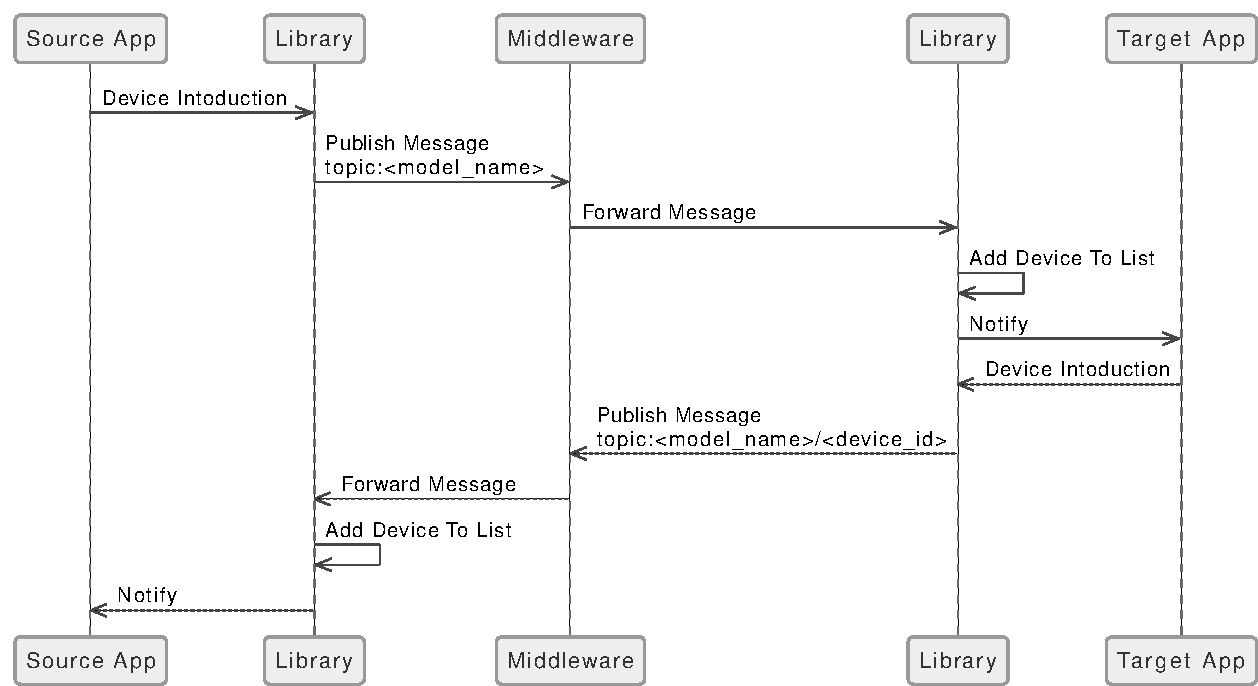
\includegraphics[width=\linewidth]{../figures/Initializing.pdf}
    \centering
    \caption{Initializing the Source Application}
    \label{fig:Initializing}
\end{figure} \FloatBarrier

\subsection{Going Offline}
An application might go offline by a user or even by other causes. A plan should cover these incidents. This step uses the Device Leave event. After disconnection, other devices are not allowed to send any message to that particular device.

\subsubsection{Graceful}
A user might close the application. In this case, the application goes offline gracefully, and it should notify other applications about its absence. Figure \ref{fig:Going-Offline-Graceful-Source} shows the source application going offline gracefully. With the library's help, the source application informs its absence to middleware on \lstinline[basicstyle=\ttfamily]{online} topic, and middleware forwards it to the library of the target application. Thereby, the library removes the device from devices list and notifies the target application about the leaving of the source application. 

\FloatBarrier \begin{figure}[H]
    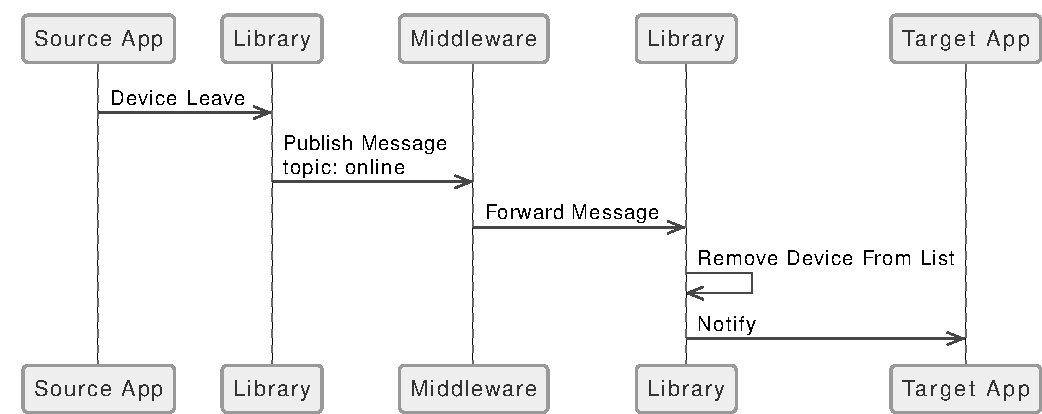
\includegraphics[width=\linewidth]{../figures/Going-Offline-Graceful-Source.pdf}
    \centering
    \caption{Going Offline Gracefully: Source}
    \label{fig:Going-Offline-Graceful-Source}
\end{figure} \FloatBarrier

\subsubsection{Ungraceful}
An application might go offline by other causes like network problems, device crashing, application failure, etc. In this case, the application goes offline ungracefully, and it should notify other applications about its absence. Figure \ref{fig:Going-Offline-Ungraceful-Source} shows the source application going offline ungracefully. The middleware checks if the application is connected; if it does not get any response, request gets a timeout and it publishes a message to  \lstinline[basicstyle=\ttfamily]{online} topic. Thereby, the library removes the device from devices list notifies the target application about the leaving of the source application.

\FloatBarrier \begin{figure}[H]
    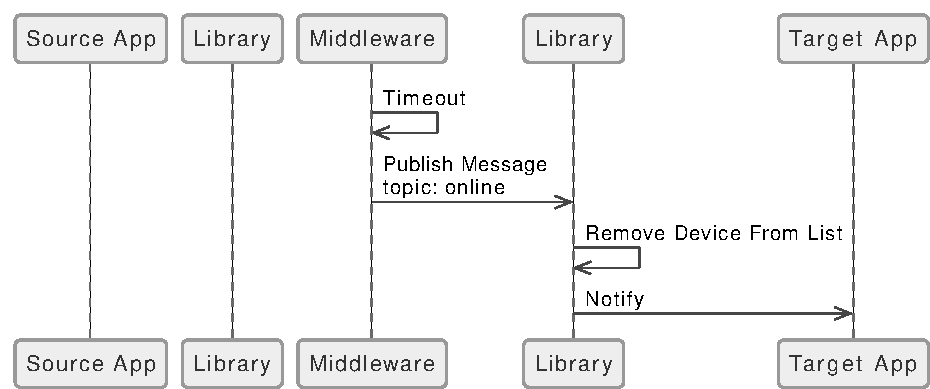
\includegraphics[width=\linewidth]{../figures/Going-Offline-Ungraceful-Source.pdf}
    \centering
    \caption{Going Offline Ungracefully: Source}
    \label{fig:Going-Offline-Ungraceful-Source}
\end{figure} \FloatBarrier

\subsubsection{Has Run-Time State}
To migrate a run-time state, an application should have a run-time state. Any application with a run-time state should notify other applications about it if they request a run-time state. This step uses the Device Has State event. Figure \ref{fig:Inform-Devices-Has-State-Source} shows the source application has a run-time state and informs the middleware by publish a message to topics of Application State Models and middleware forward it to the library of the target application. Thereby, the library notifies the target application about the source application, which has a run-time state.

\FloatBarrier \begin{figure}[H]
    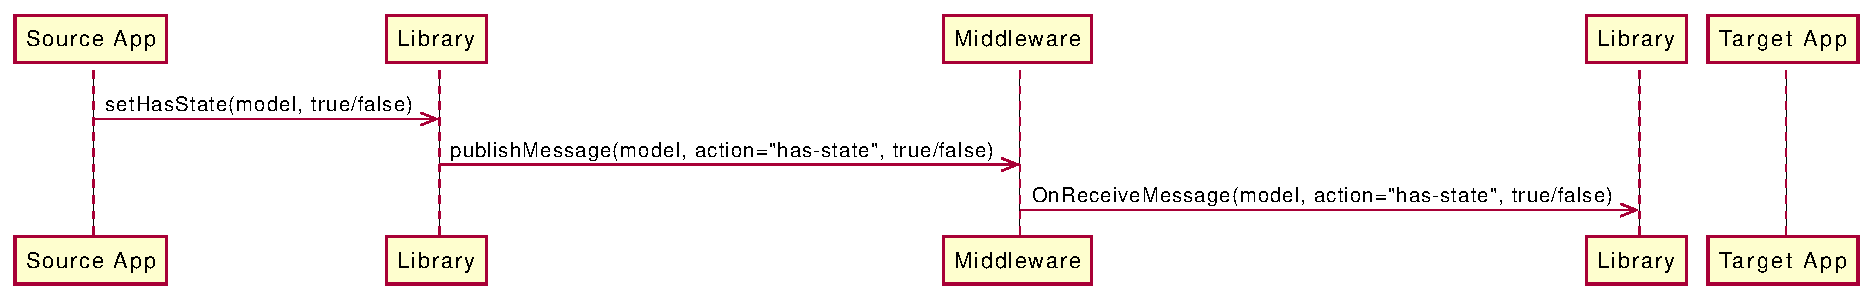
\includegraphics[width=\linewidth]{../figures/Inform-Devices-Has-State-Source.pdf}
    \centering
    \caption{Source App inform other devices that has a state}
    \label{fig:Inform-Devices-Has-State-Source}
\end{figure} \FloatBarrier

\subsection{Store Run-time State}
To migrate a run-time state of an application, it should be temporarily stored and ready for migration if other applications request it. Figure \ref{fig:Store-Current-State} shows that the source and target applications can temporarily store their run-time state in the library.

\FloatBarrier \begin{figure}[H]
    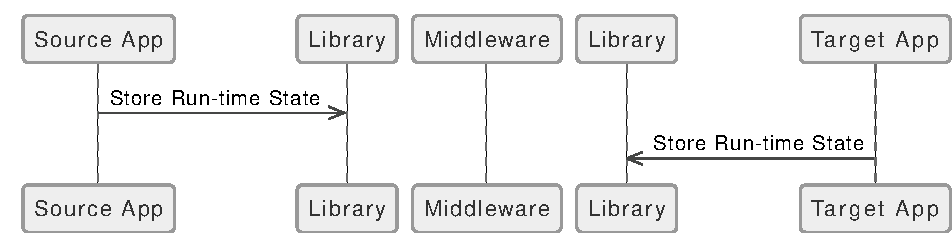
\includegraphics[width=\linewidth]{../figures/Store-Current-State.pdf}
    \centering
    \caption{Store the Current State}
    \label{fig:Store-Current-State}
\end{figure} \FloatBarrier


\subsection{Migration Patterns}
In this section, we describe two patterns for run-time state migration.

\subsubsection{Pull Method}
In the pull method, source applications request a run-time state from the target application. Figure \ref{fig:Migration-Source-to-Target-Pull-Method} shows the source application gets the list of devices with a common Application State Model, then selects the target application and requests its run-time state by sending a message from the library to middleware. The middleware forwards the message, and the target application gets a request of its run-time state. After processing the request, the target application sends its run-time state by the library to middleware. The middleware forwards the message, and the source application receives the run-time state. Source application adjusts the new run-time state and notifies the target application about finalizing the run-time state migration by sending a message to the library and middleware. 

\FloatBarrier \begin{figure}[H]
    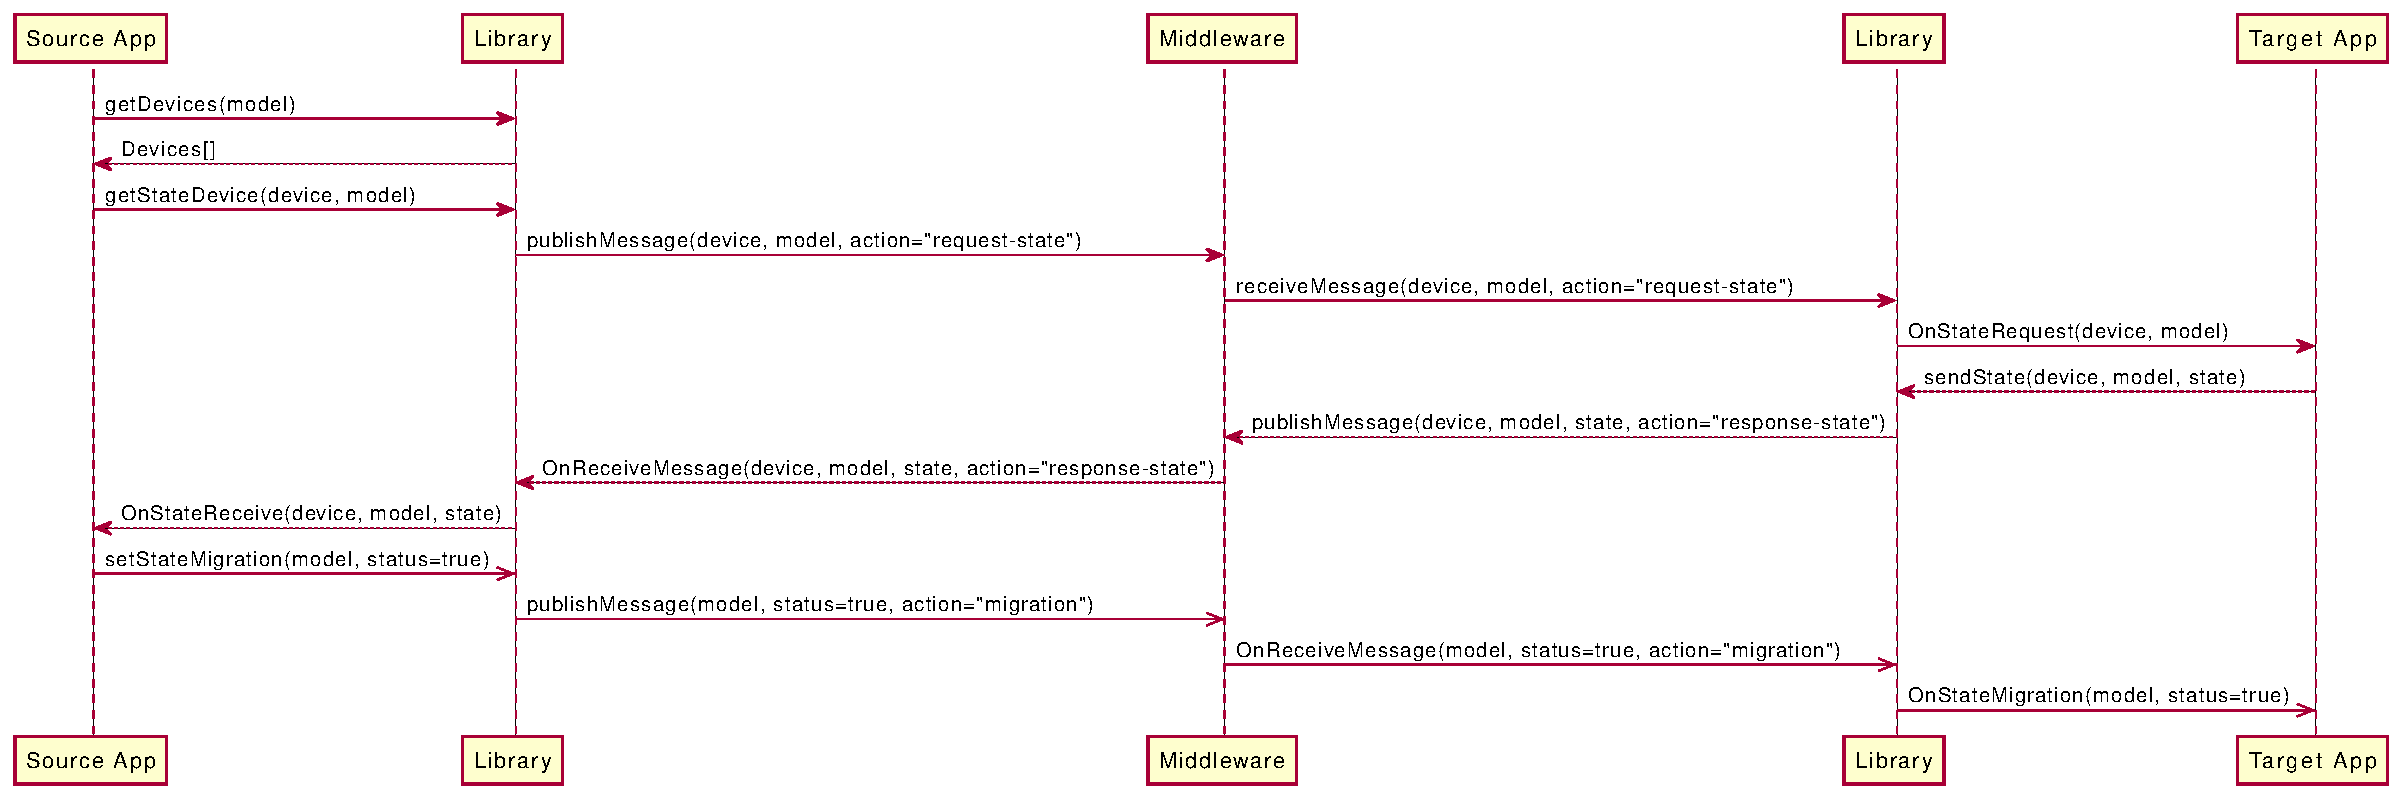
\includegraphics[width=\linewidth]{../figures/Migration-Source-to-Target-Pull-Method.pdf}
    \centering
    \caption{Pull Method: Migration Source to Target}
    \label{fig:Migration-Source-to-Target-Pull-Method}
\end{figure} \FloatBarrier

\subsubsection{Push Method}
In the push method, source applications send their run-time state to the target application without a request by force. Figure \ref{fig:Migration-Source-to-Target-Push-Method} shows the source application gets the list of devices with a common Application State Model, then selects the target application and requests its run-time state by sending a message from the library to middleware. The middleware forwards the message, and the target application gets a request of its state. After processing the request, the target application sends its run-time state by the library to middleware. The middleware forwards the message, and the source application receives the run-time state. Source application adjusts the new run-time state and notifies the target application about finalizing the run-time state migration by sending a message to the library and middleware. 

\FloatBarrier \begin{figure}[H]
    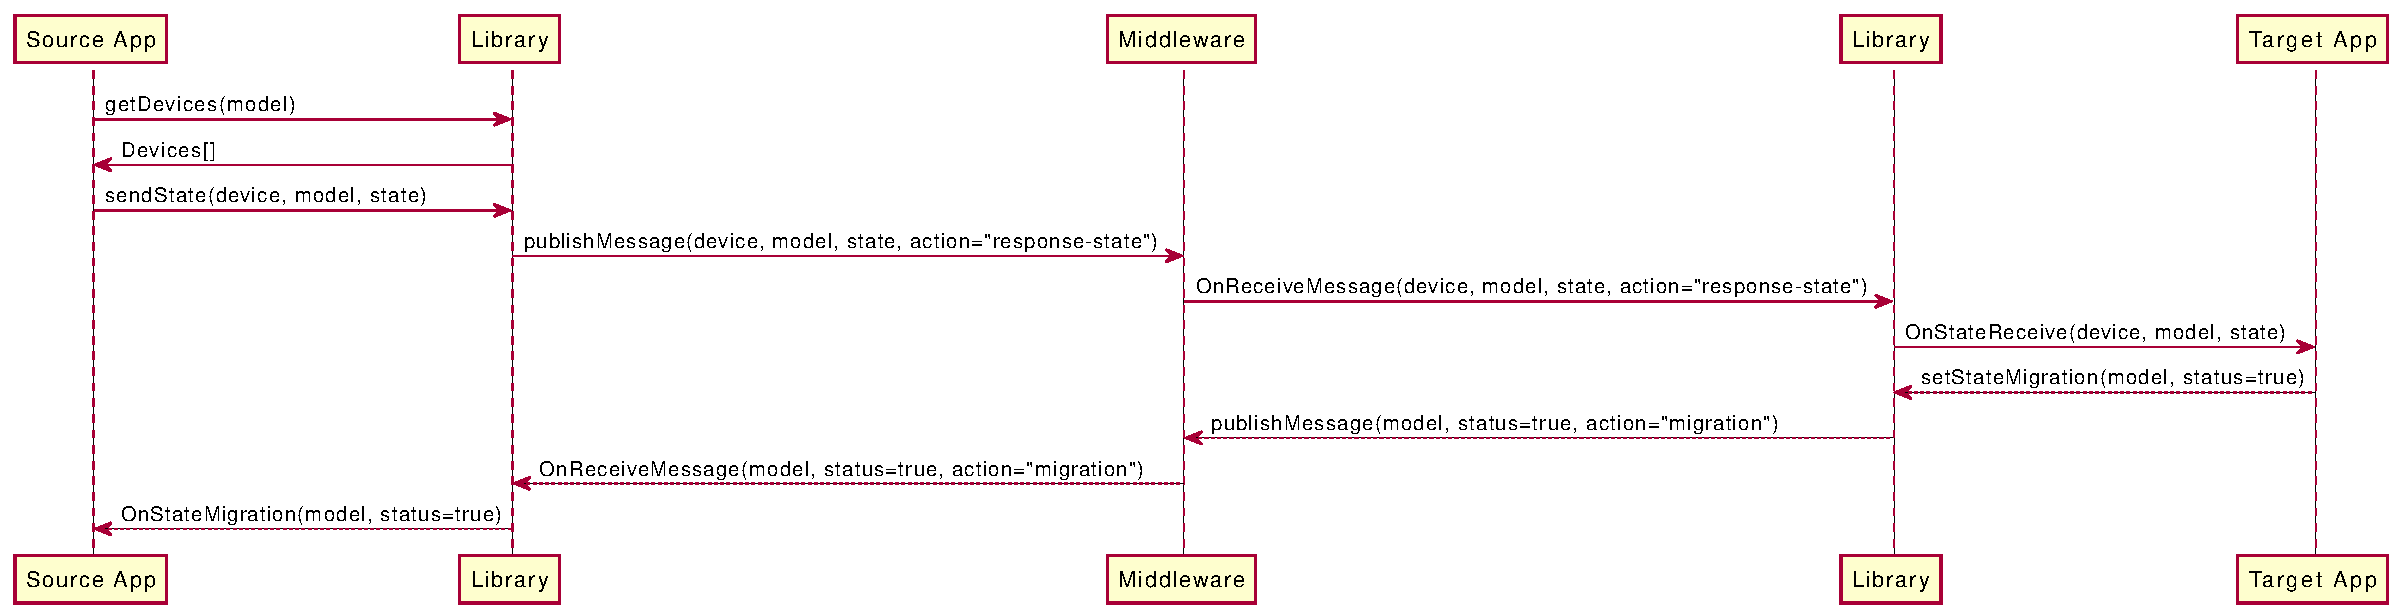
\includegraphics[width=\linewidth]{../figures/Migration-Source-to-Target-Push-Method.pdf}
    \centering
    \caption{Push Method: Migration Source to Target}
    \label{fig:Migration-Source-to-Target-Push-Method}
\end{figure} \FloatBarrier


